
% Thesis Abstract -----------------------------------------------------


%\begin{abstractslong}    %uncommenting this line, gives a different abstract heading


%\begin{abstracts}        %this creates the heading for the abstract page
%\selectlanguage{british}
% Put your abstract or summary here.

%Cuando tenemos una ecuaci\'on diferencial de grado $n$, sabemos gracias a un teorema de Cauchy que posee $n$ soluciones linealmente independientes en un punto $b \in \mathbb{C}$, si tomamos una de estas soluciones y la continuamos anal\'iticamente por un lazo anclado en $b$ obtenemos una soluci\'on que depende de las $n$ soluciones linealmente independientes dadas, gracias a este hecho, podemos de igual manera asociar un grupo a la ecuaci\'on diferencial dada, este grupo visto en $GL(2,\mathbb{C})$ contiene las matrices, llamadas matrices de conexi\'on , que relacionan a la soluci\'on original y a la continuaci\'on anal\'itica de la soluci\'on. Dado un conjunto de soluciones alrededor de un punto  $b \in \mathbb{C} $ y a la continuaci\'on anal\'itica a travez de los lazos en el grupo fundamental $\Pi_{1} (b,\mathbb{C})$ el grupo de matrices de las que se habl\'o anteriormente es llamado el grupo de monodrom\'ia.

%\begin{figure}[h]
 % \centering
  % Requires \usepackage{graphicx}
  %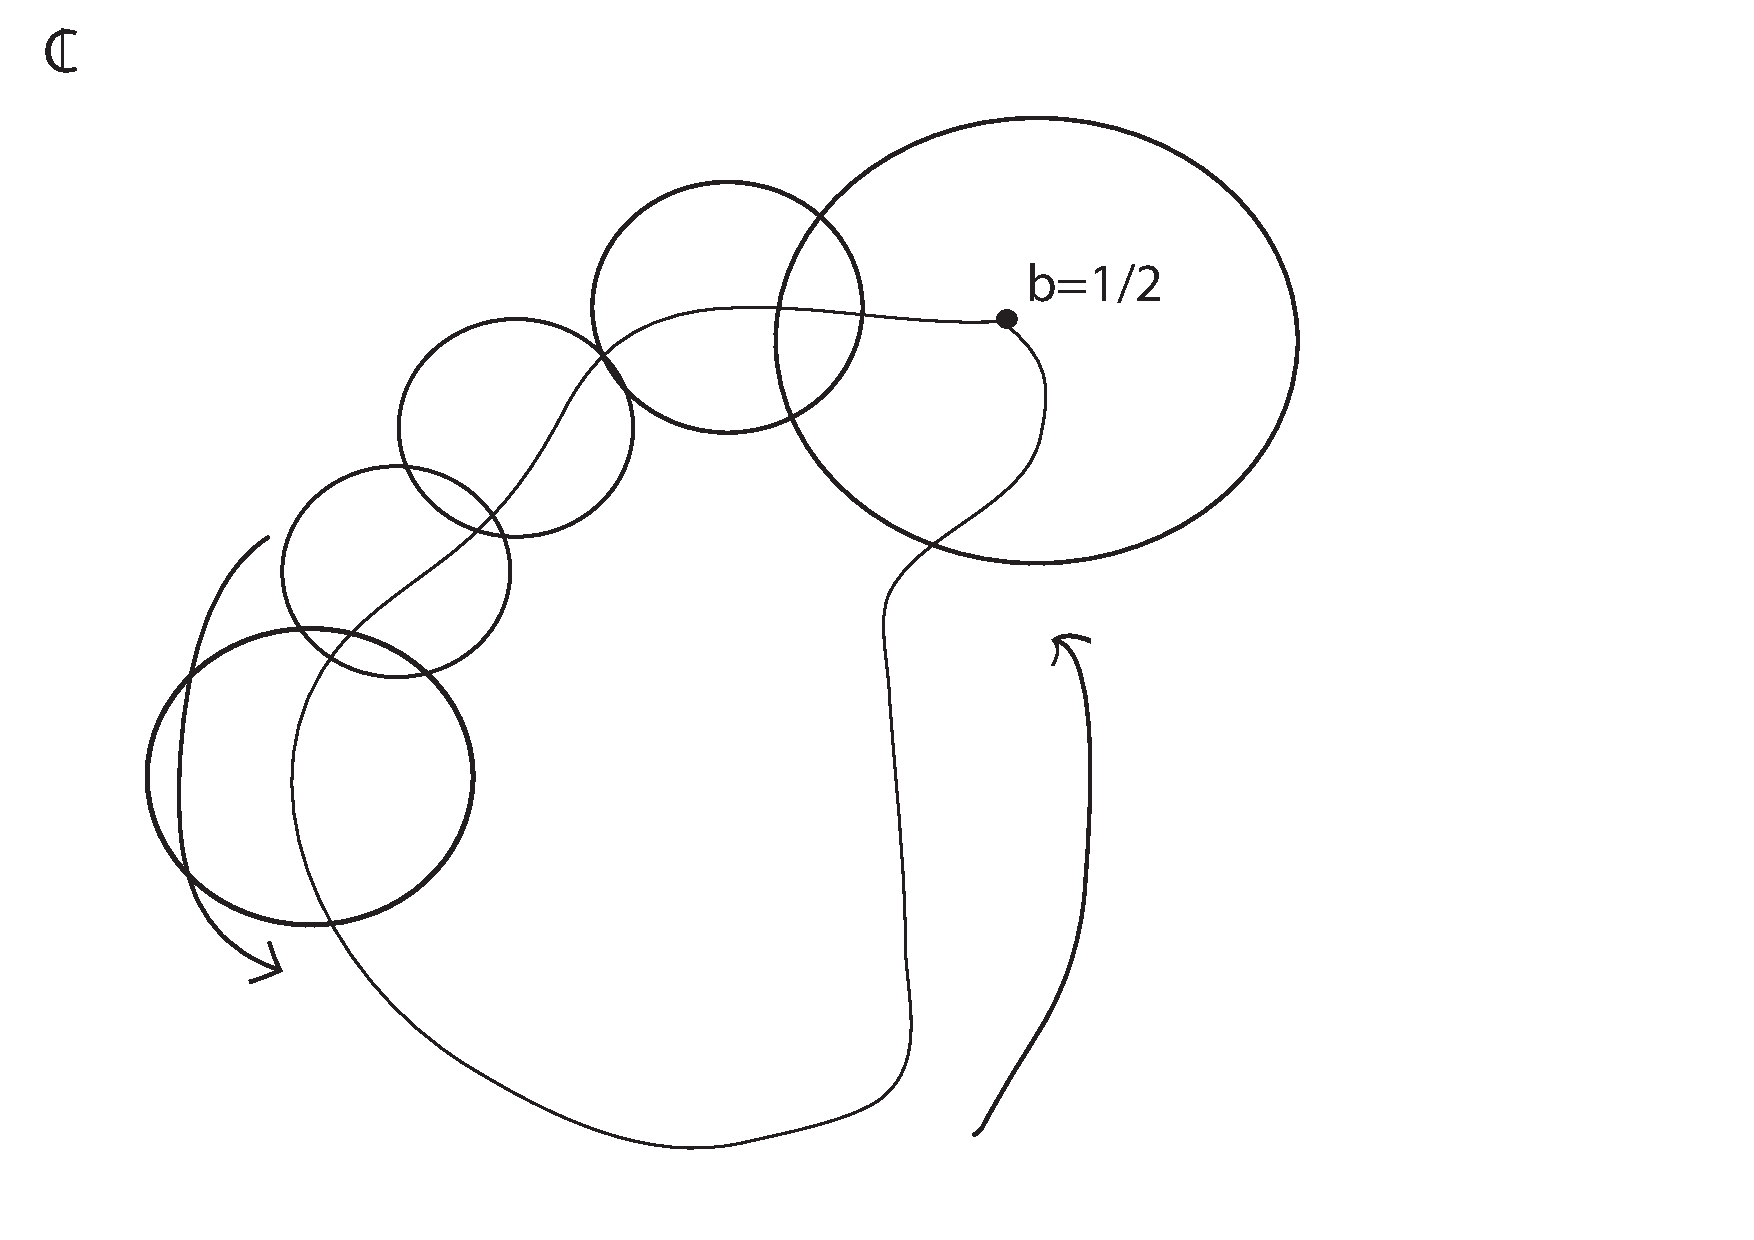
\includegraphics[width=10cm]{abstract-dibujo1}\\
  %\caption{Continuaci\'on anal\'itica}
%\end{figure}




%El grupo de monodrom\'ia nos da informaci\'on importante  de la ecuaci\'on diferencial. En general hallar la monodrom\'ia relativa a una ecuaci\'on diferencial no es una tarea sencilla . Dado este hecho, nos proponemos  hallar y dar de manera expl\'icita la monodrom\'ia y el grupo de monodrom\'ia de la ecuaci\'on diferencial hipergeom\'etrica

 %$$x(1-x)\frac{d^{2}u}{dx^{2}} +  \lbrace c- (a+b+1 )x \rbrace \frac{du}{dx} - abu=0 $$

 %Por medio de una combinaci\'on de t\'ecnicas recopiladas de numerosos textos (de manera particular en \cite{gausspainleve}), adem\'as de dar un conjunto de soluciones para esta ecuaci\'on en el punto $b=\frac{1}{2}$.\\



%El grupo de monodrom\'ia de la ecuaci\'on hipergeom\'etrica tiene una estructura de grupo de Schottky cuando tomamos los exponentes puramente imaginarios, los exponentes dados por

%$$1-c = i\theta_{0}, c-a-b = i\theta_{1},a-b=i\theta_{2} $$

%Con $\theta_{i} > 0$.

%Podemos describir la monodrom\'ia de la ecuaci\'on diferencial hipergeom\'etrica por medio de reflexiones respecto a c\'irculos $C(c,r)$ (donde $c$ es real)

%$$\psi (c,r):s \mapsto \frac{r^{2}}{\bar{s} -c} +c$$

%Y con estas reflexiones asociarle un grupo de Schottky, todo esto siguiendo los pasos de Takashi Ichikawa y Masaaki Yoshida  en una publicaci\'on titulada "ON SCHOTTKY GROUPS ARISING FROM THE HYPERGEOMETRIC EQUATION WITH IMAGINARY EXPONENTS" (\cite{Masaaki}).

%El grupo de Schottky $\Lambda_{\theta}$ asociado a la ecuaci\'on hipergeom\'etrica con exponentes imaginarios nos sirve de ejemplo en un teorema sobre grupos de isometrias del plano hiperb\'olico que act\'uan de manera discontinua en el cual se destaca su prueba casi completamente geom\'etrica propuesta en un art\'iculo de W. Fenchel y J. Nielsen llamado "ON DISCONTINOUS GROUPS OF ISOMETRIC TRANSFORMATIONS OF THE NON-EUCLIDIAN PLANE" publicado en el año de 1948 (\cite{Nielsen}), aunque dado que tenemos 3 parametros $\theta_{1},\theta_{2},\theta_{3}$, en realidad hemos dado muchos ejemplos que cumplen de igual manera este prop\'osito.


%Para obtener este resultado usamos la noci\'on de grupo \textit{elemental} que definimos enseguida.

%\begin{defn}
%\label{def:elemental}
%Un grupo es elemental si su conjunto l\'imite esta formado a lo m\'as por dos puntos
%\end{defn}

%La caracteristica que realmente es de \'interes para nosotros es que un grupo sea NO-elemental, dicho grupo es por lo tanto un grupo cuyo conjunto l\'imite esta formado por  mas de dos puntos.
%En \cite{Nielsen} tenemos la siguiente definici\'on;

%\begin{defn}
%\label{def:discontinuo2}
%Un grupo $G$ se dice discontinuo en un punto $x \in \mathbb{D}$ si $x$ no es un punto de acumulaci\'on de la clase $Gx$
%\end{defn}

%Nuestro objetivo es encontrar ejemplos de grupos que actuen de manera discontinua en $\mathbb{D}$ y verificar en ellos las condiciones del teorema de Nielsen. Los grupos de Schottky que hallamos son discretos y adem\'as son No-elementales estas caracteristicas implican que se cumple en $\mathbb{D}$ la siguiente definici\'on;



%\begin{defn}
%\label{def:discontinuo1}
%Sea $X$ un espacio topologico arbitrario y $G$ un grupo de homeomorfismos de $X$ en $X$. Se dice que $G$ act\'ua discontinuamente en $X$ si y solo si para cada subconjunto compacto $K$ de $X$ se tiene,

%$$g(K) \cap K = \emptyset $$

%Excepto para un n\'umero finito de $g$'s en $G$
%\end{defn}

%Los ejemplos que encontramos satisfacen lo que deseamos gracias a un teorema que podemos encontrar en  \cite{Beardon}, pero tambi\'en gracias a que \ref{def:discontinuo1} implica \ref{def:discontinuo2}, de esta manera sabemos de antemano que nuestros grupos act\'uan de manera discontinua pero tambi\'en nos interesa indagar las condiciones que el teorema de Nielsen requiere y deducir algunas propiedades ya que la demostraci\'on de este teorema en \cite{Nielsen} aclara el comportamiento geom\'etrico de los grupos de transformaciones hiperb\'olicas.




%\end{abstracts}

\begin{resumen}        %this creates the heading for the abstract page
\selectlanguage{spanish}

\renewcommand\baselinestretch{3}

Cuando tenemos una ecuaci\'on diferencial de grado $n$, sabemos gracias a un teorema de Cauchy que posee $n$ soluciones linealmente independientes en un punto $b \in \mathbb{C}$, si tomamos una de estas soluciones y la continuamos anal\'iticamente por un lazo anclado en $b$ obtenemos una soluci\'on que depende de las $n$ soluciones linealmente independientes dadas, gracias a este hecho, podemos de igual manera asociar un grupo a la ecuaci\'on diferencial dada, este grupo visto en $GL(2,\mathbb{C})$ contiene las matrices, llamadas matrices de conexi\'on , que relacionan a la soluci\'on original y a la continuaci\'on anal\'itica de la soluci\'on. Dado un conjunto de soluciones alrededor de un punto  $b \in \mathbb{C} $ y a la continuaci\'on anal\'itica a travez de los lazos en el grupo fundamental $\Pi_{1} (b,\mathbb{C})$ el grupo de matrices de las que se habl\'o anteriormente es llamado el grupo de monodrom\'ia.

\begin{figure}[h]
  \centering
  % Requires \usepackage{graphicx}
  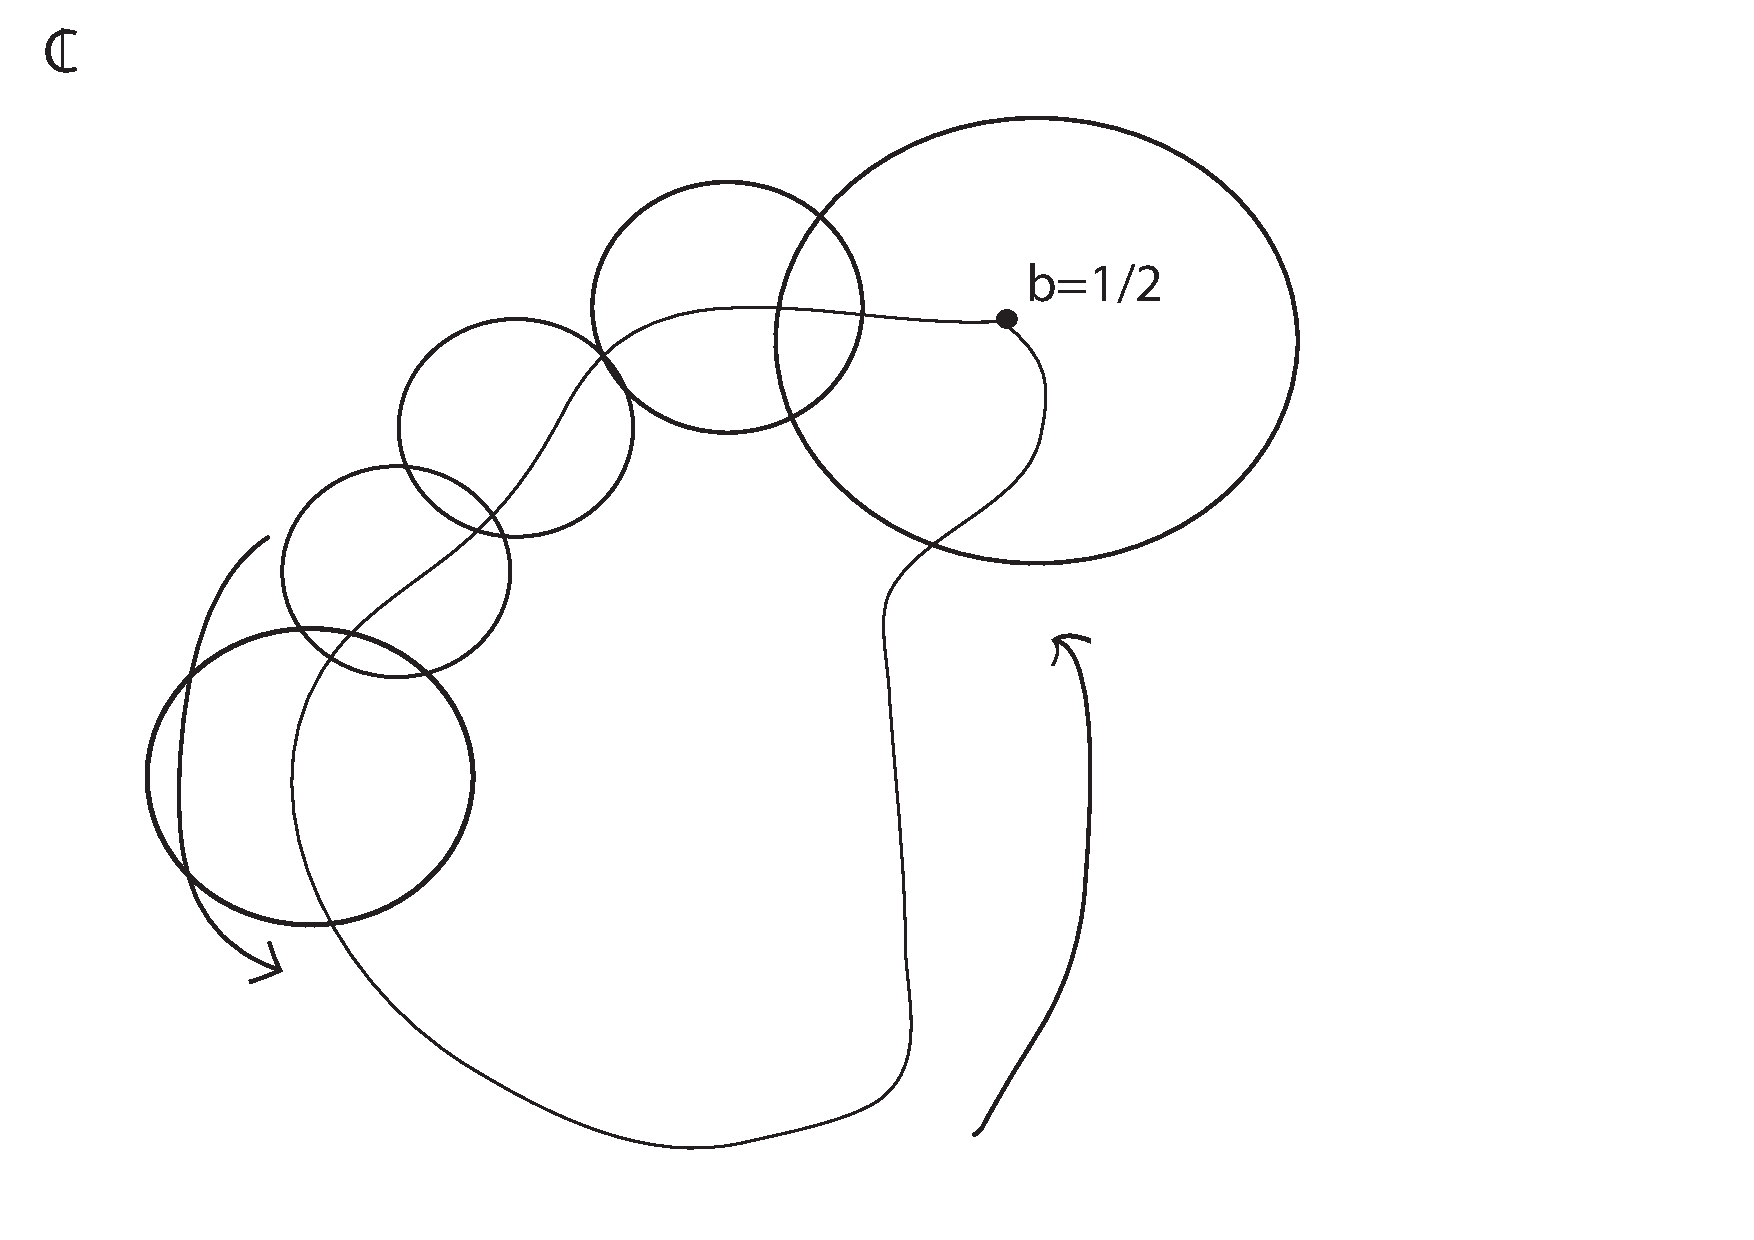
\includegraphics[width=10cm]{abstract-dibujo1.pdf}\\
  \caption{Continuaci\'on anal\'itica}
\end{figure}




El grupo de monodrom\'ia nos da informaci\'on importante  de la ecuaci\'on diferencial. En general hallar la monodrom\'ia relativa a una ecuaci\'on diferencial no es una tarea sencilla . %Dado este hecho,   
Nos proponemos  hallar y dar de manera expl\'icita %la monodrom\'ia y
el grupo de monodrom\'ia de la ecuaci\'on diferencial hipergeom\'etrica.

 $$x(1-x)\frac{d^{2}u}{dx^{2}} +  \lbrace c- (a+b+1 )x \rbrace \frac{du}{dx} - abu=0 $$

 Por medio de una combinaci\'on de t\'ecnicas recopiladas de numerosos textos (de manera particular en \cite{gausspainleve}), adem\'as de dar un conjunto de soluciones para esta ecuaci\'on en el punto $b=\frac{1}{2}$.\\



El grupo de monodrom\'ia de la ecuaci\'on hipergeom\'etrica tiene una estructura de grupo de Schottky cuando tomamos los exponentes puramente imaginarios, los exponentes dados por

$$1-c = i\theta_{0}, c-a-b = i\theta_{1},a-b=i\theta_{2} $$

Con $\theta_{i} > 0$.

Podemos describir la monodrom\'ia de la ecuaci\'on diferencial hipergeom\'etrica por medio de reflexiones respecto a c\'irculos $C(c,r)$ (donde $c$ es real)

$$\psi (c,r):s \mapsto \frac{r^{2}}{\bar{s} -c} +c$$

Y con estas reflexiones asociarle un grupo de Schottky, todo esto siguiendo los pasos de Takashi Ichikawa y Masaaki Yoshida  en una publicaci\'on titulada "ON SCHOTTKY GROUPS ARISING FROM THE HYPERGEOMETRIC EQUATION WITH IMAGINARY EXPONENTS" (\cite{Masaaki}).

El grupo de Schottky $\Lambda_{\theta}$ asociado a la ecuaci\'on hipergeom\'etrica con exponentes imaginarios nos sirve de ejemplo en un teorema sobre grupos de isometrias del plano hiperb\'olico que act\'uan de manera discontinua en el cual se destaca su prueba casi completamente geom\'etrica propuesta en un art\'iculo de W. Fenchel y J. Nielsen llamado "ON DISCONTINOUS GROUPS OF ISOMETRIC TRANSFORMATIONS OF THE NON-EUCLIDIAN PLANE" publicado en el año de 1948 (\cite{Nielsen}), aunque dado que tenemos 3 parametros $\theta_{1},\theta_{2},\theta_{3}$, en realidad hemos dado muchos ejemplos que cumplen de igual manera este prop\'osito.


Para obtener este resultado usamos la noci\'on de grupo \textit{elemental} que definimos enseguida.

\begin{defn}
\label{def:elemental}
Un grupo es elemental si su conjunto l\'imite esta formado a lo m\'as por dos puntos
\end{defn}

La caracteristica que realmente es de \'interes para nosotros es que un grupo sea NO-elemental, dicho grupo es por lo tanto un grupo cuyo conjunto l\'imite esta formado por  mas de dos puntos.
En \cite{Nielsen} tenemos la siguiente definici\'on;

\begin{defn}
\label{def:discontinuo2}
Un grupo $G$ se dice discontinuo en un punto $x \in \mathbb{D}$ si $x$ no es un punto de acumulaci\'on de la clase $Gx$
\end{defn}

Nuestro objetivo es encontrar ejemplos de grupos que actuen de manera discontinua en $\mathbb{D}$ y verificar en ellos las condiciones del teorema de Nielsen. Los grupos de Schottky que hallamos son discretos y adem\'as son No-elementales estas caracteristicas implican que se cumple en $\mathbb{D}$ la siguiente definici\'on;



\begin{defn}
\label{def:discontinuo1}
Sea $X$ un espacio topologico arbitrario y $G$ un grupo de homeomorfismos de $X$ en $X$. Se dice que $G$ act\'ua discontinuamente en $X$ si y solo si para cada subconjunto compacto $K$ de $X$ se tiene,

$$g(K) \cap K = \emptyset $$

Excepto para un n\'umero finito de $g$'s en $G$
\end{defn}

Los ejemplos que encontramos satisfacen lo que deseamos gracias a un teorema que podemos encontrar en  \cite{Beardon}, pero tambi\'en gracias a que \ref{def:discontinuo1} implica \ref{def:discontinuo2}, de esta manera sabemos de antemano que nuestros grupos act\'uan de manera discontinua pero tambi\'en nos interesa indagar las condiciones que el teorema de Nielsen requiere y deducir algunas propiedades ya que la demostraci\'on de este teorema en \cite{Nielsen} aclara el comportamiento geom\'etrico de los grupos de transformaciones hiperb\'olicas.

El cap\'itulo 1 y 2 nos dan las bases para el desarrollo de este trabajo. El cap\'itulo 1 esta basado en las definiciones necesarias como continuación anal\'itica , grupos Klenianos y de Schottky as\'i como una  introducción de la ecuación diferencial hipergeom\'etrica.

En el cap\'itulo 2 hablamos de la monodrom\'ia en general, el esquema de Riemann, calculamos la monodrom\'ia de la ecuaci\'on hipergemo\'etrica y hallamos el grupo de monodrom\'ia con las soluciones dadas por la serie hipergeom\'etrica.


En el cap\'itulo 3 construimos el grupo de schottky asociado al grupo de monodrom\'ia a trav\'es de los dominios fundamentales dados en (\cite{Masaaki})dicho grupo generado por reflexiones nos servira como ejemplo para el teorema principal.

En el cap\'itulo 4 probamos el teorema de Nielsen en 2 partes, la primera parte se prueba de manera sencilla bajo el supuesto de que en el grupo $G<PSL(2,\mathbb{R})$ existen elementos el\'ipticos, la segunda parte supone que no existen elementos el\'ipticos en el grupo y se utilizan 5 lemas para probar el teorema, estos lemas destacan mayormente por sus demostraciones puramente geom\'etricas asi como la demostraci\'on del teorema, al final probamos que el grupo de Schottky encontrado aplica en el teorema de Nielsen.      



\end{resumen}


%\begin{laburpena}        %this creates the heading for the abstract page
%\selectlanguage{basque}
% Jarri zure laburpena hemen.
%\end{laburpena}

%\end{abstractlongs}


% ----------------------------------------------------------------------
